\beginsong{Ye Jacobites}[
    wuw={Robert Burns, Musik aus Schottland}, 
    pfiii={96}, 
    pfii={188}, 
    bo={436}, 
    kssiv={132}, siru={297},
]

\beginchorus
\endchorus
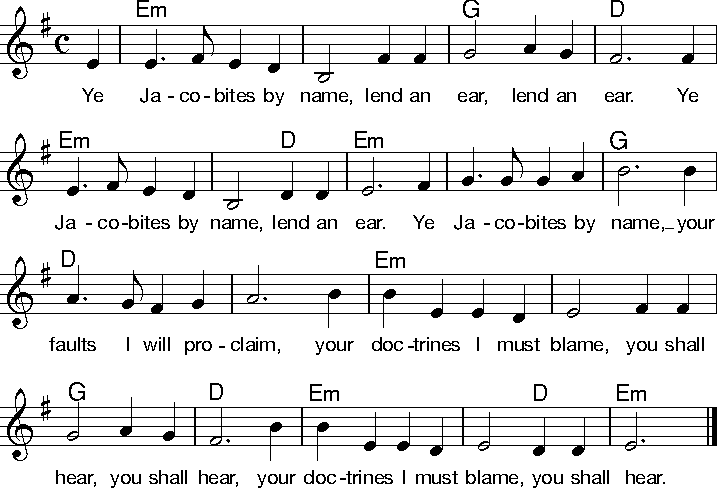
\includegraphics[draft=false, width=1\textwidth]{Noten/Lied103.pdf}	

\beginverse
What's \[Em]right and what is wrong, by the \[G]law, by the \[D]law?
what's \[Em]right and what is wrong, \[D]by the \[Em]law?
What's right and what is \[G]wrong, a \[D]short sword or a long,
a \[Em]weak arm or a strong, for to \[G]draw, for to \[D]draw.
A \[Em]weak arm or a strong, \[D]for to \[Em]draw.
\endverse

\printchorus

\beginverse
What ^makes heroic strife, famed a^far, famed a^far?
What ^makes heroic strife, ^famed a^far?
What makes heroic ^strife, to ^whet assassin's knife?
or ^haunt a parent's life neith bloody ^war, bloody ^war.
Or ^haunt a parent's life neith ^bloody ^war.
\endverse

\printchorus

\beginverse
Then ^leave your schemes alone, in the ^state, in the ^state,
then ^leave your schemes alone, ^in the ^state.
Then leave you schemes a^lone, and a^dore the rising sun
and ^leave a man undone to his ^faith, to his ^faith.
And ^leave a man undone ^to his ^faith.
\endverse

\printchorus

\endsong

\beginscripture{}
Ye Jacobites ist ein traditionelles schottisches Volkslied. Es geht auf die 'Jacobite Risings', eine Reihe von Aufständen in Großbritannien und Irland zwischen 1688 und 1746, zurück.
\endscripture
